\documentclass[a4paper,10pt]{article}
\usepackage[brazilian]{babel}
\usepackage[left=2.5cm,right=2.5cm,top=3cm,bottom=2.5cm]{geometry}
\usepackage{mathtools}
\usepackage{amsthm}
\usepackage{amsmath}
%\usepackage{nccmath}
\usepackage{amssymb}
\usepackage{amsfonts}
\usepackage{physics}
%\usepackage{dsfont}
%\usepackage{mathrsfs}

\usepackage{titling}
\usepackage{indentfirst}

\usepackage{bm}
\usepackage[dvipsnames]{xcolor}
\usepackage{cancel}

\usepackage{xurl}
\usepackage[colorlinks=true]{hyperref}

\usepackage{float}
\usepackage{graphicx}
%\usepackage{tikz}
\usepackage{caption}
\usepackage{subcaption}

%%%%%%%%%%%%%%%%%%%%%%%%%%%%%%%%%%%%%%%%%%%%%%%%%%%

\newcommand{\eps}{\epsilon}
\newcommand{\vphi}{\varphi}
\newcommand{\cte}{\text{cte}}

\newcommand{\N}{\mathbb{N}}
\newcommand{\Z}{\mathbb{Z}}
\newcommand{\Q}{\mathbb{Q}}
\newcommand{\R}{\vb{R}}
\newcommand{\C}{\mathbb{C}}
\renewcommand{\S}{\hat{S}}
%\renewcommand{\H}{\s{H}}

\renewcommand{\a}{\vb{a}}
\newcommand{\nn}{\hat{n}}
\renewcommand{\d}{\dagger}
\newcommand{\up}{\uparrow}
\newcommand{\down}{\downarrow}

\newcommand{\0}{\vb{0}}
%\newcommand{\1}{\mathds{1}}
\newcommand{\E}{\vb{E}}
\newcommand{\B}{\vb{B}}
\renewcommand{\v}{\vb{v}}
\renewcommand{\r}{\vb{r}}
\renewcommand{\k}{\vb{k}}
\newcommand{\p}{\vb{p}}
\newcommand{\q}{\vb{q}}
\newcommand{\F}{\vb{F}}

\newcommand{\s}{\sigma}
%\newcommand{\prodint}[2]{\left\langle #1 , #2 \right\rangle}
\newcommand{\cc}[1]{\overline{#1}}
\newcommand{\Eval}[3]{\eval{\left( #1 \right)}_{#2}^{#3}}

\newcommand{\unit}[1]{\; \mathrm{#1}}

\newcommand{\n}{\medskip}
\newcommand{\e}{\quad \mathrm{e} \quad}
\newcommand{\ou}{\quad \mathrm{ou} \quad}
\newcommand{\virg}{\, , \;}
\newcommand{\ptodo}{\forall \,}
\renewcommand{\implies}{\; \Rightarrow \;}
%\newcommand{\eqname}[1]{\tag*{#1}} % Tag equation with name

\setlength{\droptitle}{-7em}

\theoremstyle{plain}
\newtheorem{theorem}{Teorema}[section]
%\newtheorem{defi}[theorem]{Definição}
\newtheorem{lemma}[theorem]{Lema}
%\newtheorem{corol}[theorem]{Corolário}
%\newtheorem{prop}[theorem]{Proposição}
%\newtheorem{example}{Exemplo}
%
%\newtheorem{inneraxiom}{Axioma}
%\newenvironment{axioma}[1]
%  {\renewcommand\theinneraxiom{#1}\inneraxiom}
%  {\endinneraxiom}
%
%\newtheorem{innerpostulado}{Postulado}
%\newenvironment{postulado}[1]
%  {\renewcommand\theinnerpostulado{#1}\innerpostulado}
%  {\endinnerpostulado}
%
%\newtheorem{innerexercise}{Exercício}
%\newenvironment{exercise}[1]
%  {\renewcommand\theinnerexercise{#1}\innerexercise}
%  {\endinnerexercise}
%
%\newtheorem{innerthm}{Teorema}
%\newenvironment{teorema}[1]
%  {\renewcommand\theinnerthm{#1}\innerthm}
%  {\endinnerthm}
%
\newtheorem{innerlema}{Lema}
\newenvironment{lema}[1]
  {\renewcommand\theinnerlema{#1}\innerlema}
  {\endinnerlema}
%
%\theoremstyle{remark}
%\newtheorem*{hint}{Dica}
%\newtheorem*{notation}{Notação}
%\newtheorem*{obs}{Observação}


\renewcommand{\p}{\phantom{+}}
\newcommand{\mchi}{\chi^{\Gamma^\pi_{p_z}}}
\renewcommand{\c}[1]{\textcolor{red}{#1}}

\title{\Huge{\textbf{Teoria de grupos - Exercício 3}}}
\author{Mateus Marques}

\begin{document}

\maketitle

\section*{Enunciado}

\begin{itemize}
\item encontrar o grupo de simetria da molécula (descrever ou desenhar todos os elementos de simetria)

\item dados os orbitais $p_z$ dos seis átomos de carbono que formam os orbitais moleculares $\pi$, encontrar a representação $\Gamma_{p_z}^\pi$ \implies
traços das matrizes dos operadores de transformação dos orbitais $p_z$ $(\vphi_1, \vphi_2, \vphi_3, \vphi_4, \vphi_5, \vphi_6)$.

\item encontrar com que representações irredutíveis do grupo da molécula os orbitais $p_z$ se transformam

\item obter os orbitais simetrizados (e normalizados) da molécula \implies aplicar dos operadores de projeção para obter as funções projetadas nos subespaços das representações irredutíveis.
\end{itemize}


\section*{A ligação $\pi$ da molécula de benzeno C$_6$H$_6$}

A molécula de benzeno tem geometria de um hexágono. Assim, ela possui um eixo $C_6$ (o eixo $z$), 6 eixos $C_2$ (no plano da molécula, 3 passando pelos átomos de carbono e 3 passando pelo meio das arestas do hexágono) e, além disso, ela também possui um plano de reflexão $\sigma_h$. No total, isso totaliza $12 \cdot 2 = 24$ elementos. Note que essas características correspondem unicamente ao grupo $D_{6h} = D_6 \otimes C_{1h}$.

\begin{figure}[H]
\centering
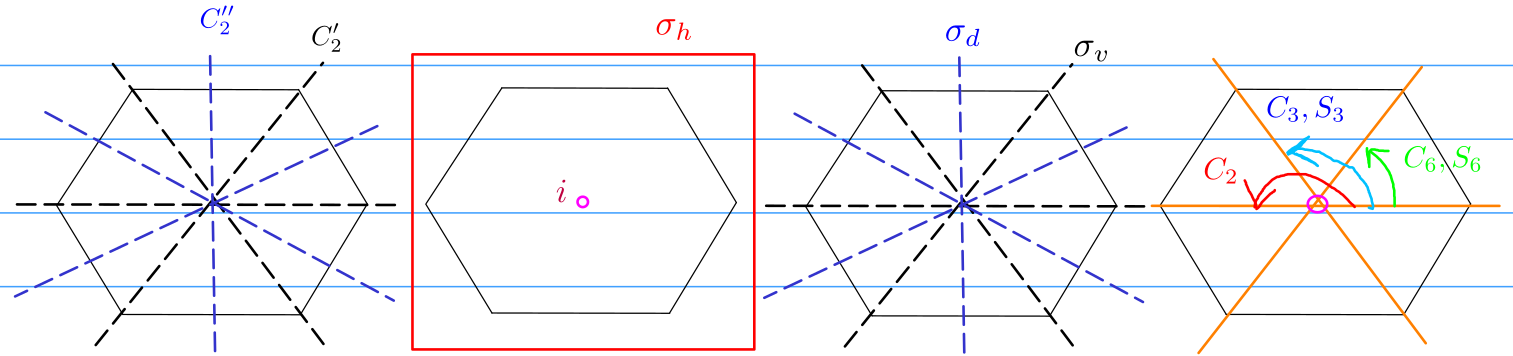
\includegraphics[width=1.0\linewidth]{fig/D6h.png}
\caption{Elementos de simetria do grupo $D_{6h}$, correspondente à molécula de benzeno C$_6$H$_6$.}
\label{fig:D6h}
\end{figure}

Agora descobriremos a representação $\Gamma^\pi_{p_z}$. Note que a base tem dimensão $6$, já que temos 6 orbitais, representados pelo vetor $(\vphi_1, \vphi_2, \vphi_3, \vphi_4, \vphi_5, \vphi_6)$. Avaliaremos os caracteres dessa representação $\Gamma^\pi_{p_z}$ para seus elementos, seguindo os desenhos da Figura \ref{fig:D6h}:
\begin{enumerate}
\item $E$ $\implies$ matriz identidade de dimensão 6, portanto $\mchi(E) = 6$.
\item $C_6$ (eixo $z$) $\implies$ troca os 6 orbitais de lugar, portanto $\mchi(C_6) = 0$.
\item $C_3$ (eixo $z$) $\implies$ troca os 6 orbitais de lugar, portanto $\mchi(C_3) = 0$.
\item $C_2$ (eixo $z$) $\implies$ troca os 6 orbitais de lugar, portanto $\mchi(C_2) = 0$.
\item $C_2'$ $\implies$ mantém 2 dos 6 orbitais inalterados e inverte a polarização, portanto $\mchi(C_2') = -2$.
\item $C_2''$ $\implies$ troca os 6 orbitais de lugar, portanto $\mchi(C_2'') = 0$.
\item $i$ $\implies$ troca os 6 orbitais de lugar, portanto $\mchi(i) = 0$.
\item $S_3$ $\implies$ troca os 6 orbitais de lugar, portanto $\mchi(S_3) = 0$.
\item $S_6$ $\implies$ troca os 6 orbitais de lugar, portanto $\mchi(S_6) = 0$.
\item $\sigma_h$ $\implies$ mantém os 6 orbitais, mas inverte a polarização de todos, portanto $\mchi(\sigma_h) = -6$.
\item $\sigma_d$ $\implies$ troca os 6 orbitais de lugar, portanto $\mchi(\sigma_d) = 0$.
\item $\sigma_v$ $\implies$ mantém 2 dos 6 orbitais e mantém a polarização, portanto $\mchi(\sigma_v) = 2$.
\end{enumerate}

Retirando a tabela de caracter do site \url{http://symmetry.jacobs-university.de/cgi-bin/group.cgi?group=606&option=4}.

\begin{table}[H]
\caption{Tabela de caracteres para o grupo $D_{6h}$.}
\centering

\begin{tabular} { |c|c c c c c c c c c c c c | }
\hline
$D_{6h}$ & $E$ & $2 C_6$ & $2 C_3$ & $C_2$ & $3 C_2'$ & $3 C_2''$ & $i$ & $2 S_3$ & $2 S_6$ & $\sigma_h$ & $3 \sigma_d$ & $3 \sigma_v$ \\
\hline
$A_{1g}$ & $\p1$ & $\p1$ & $\p1$ & $\p1$ & $\p1$ & $\p1$ & $\p1$ & $\p1$ & $\p1$ & $\p1$ & $\p1$ & $\p1$ \\
$A_{2g}$ & $\p1$ & $\p1$ & $\p1$ & $\p1$ & $ -1$ & $ -1$ & $\p1$ & $\p1$ & $\p1$ & $\p1$ & $ -1$ & $ -1$ \\
$B_{1g}$ & $\p1$ & $ -1$ & $\p1$ & $ -1$ & $\p1$ & $ -1$ & $\p1$ & $ -1$ & $\p1$ & $ -1$ & $\p1$ & $ -1$ \\
$\c{\boxed{B_{2g}}}$ & $\c{\p1}$ & $\c{ -1}$ & $\c{\p1}$ & $\c{ -1}$ & $\c{ -1}$ & $\c{\p1}$ & $\c{\p1}$ & $\c{ -1}$ & $\c{\p1}$ & $\c{ -1}$ & $\c{ -1}$ & $\c{\p1}$ \\
$\c{\boxed{E_{1g}}}$ & $\c{\p2}$ & $\c{\p1}$ & $\c{ -1}$ & $\c{ -2}$ & $\c{\p0}$ & $\c{\p0}$ & $\c{\p2}$ & $\c{\p1}$ & $\c{ -1}$ & $\c{ -2}$ & $\c{\p0}$ & $\c{\p0}$ \\
$E_{2g}$ & $\p2$ & $ -1$ & $ -1$ & $\p2$ & $\p0$ & $\p0$ & $\p2$ & $ -1$ & $ -1$ & $\p2$ & $\p0$ & $\p0$ \\
$A_{1u}$ & $\p1$ & $\p1$ & $\p1$ & $\p1$ & $\p1$ & $\p1$ & $ -1$ & $ -1$ & $ -1$ & $ -1$ & $ -1$ & $ -1$ \\
$\c{\boxed{A_{2u}}}$ & $\c{\p1}$ & $\c{\p1}$ & $\c{\p1}$ & $\c{\p1}$ & $\c{ -1}$ & $\c{ -1}$ & $\c{ -1}$ & $\c{ -1}$ & $\c{ -1}$ & $\c{ -1}$ & $\c{\p1}$ & $\c{\p1}$ \\
$B_{1u}$ & $\p1$ & $ -1$ & $\p1$ & $ -1$ & $\p1$ & $ -1$ & $ -1$ & $\p1$ & $ -1$ & $\p1$ & $ -1$ & $\p1$ \\
$B_{2u}$ & $\p1$ & $ -1$ & $\p1$ & $ -1$ & $ -1$ & $\p1$ & $ -1$ & $\p1$ & $ -1$ & $\p1$ & $\p1$ & $ -1$ \\
$E_{1u}$ & $\p2$ & $\p1$ & $ -1$ & $ -2$ & $\p0$ & $\p0$ & $ -2$ & $ -1$ & $\p1$ & $\p2$ & $\p0$ & $\p0$ \\
$\c{\boxed{E_{2u}}}$ & $\c{\p2}$ & $\c{ -1}$ & $\c{ -1}$ & $\c{\p2}$ & $\c{\p0}$ & $\c{\p0}$ & $\c{ -2}$ & $\c{\p1}$ & $\c{\p1}$ & $\c{ -2}$ & $\c{\p0}$ & $\c{\p0}$ \\
\hline
\hline
$\Gamma_{p_z}^\pi$ & $\p6$ & $\p0$ & $\p0$ & $\p0$ & $ -2$ & $\p0$ & $\p0$ & $\p0$ & $\p0$ & $ -6$ & $\p0$ & $\p2$ \\
\hline
\end{tabular}

\label{tab:mult_D3h}
\end{table}

Temos portanto que
$$
\Gamma^\pi_{p_z} = B_{2g} \oplus E_{1g} \oplus A_{2u} \oplus E_{2u}.
$$

Agora basta aplicar os operadores de projeção para obter os orbitais simetrizados.

B2g
$$
\frac{\sqrt{6} \varphi_{1}}{6} - \frac{\sqrt{6} \varphi_{2}}{6} + \frac{\sqrt{6} \varphi_{3}}{6} - \frac{\sqrt{6} \varphi_{4}}{6} + \frac{\sqrt{6} \varphi_{5}}{6} - \frac{\sqrt{6} \varphi_{6}}{6}
$$

E1g
$$
\frac{\sqrt{3} \varphi_{1}}{3} + \frac{\sqrt{3} \varphi_{2}}{6} - \frac{\sqrt{3} \varphi_{3}}{6} - \frac{\sqrt{3} \varphi_{4}}{3} - \frac{\sqrt{3} \varphi_{5}}{6} + \frac{\sqrt{3} \varphi_{6}}{6}
$$
$$
\frac{\varphi_{2}}{2} + \frac{\varphi_{3}}{2} - \frac{\varphi_{5}}{2} - \frac{\varphi_{6}}{2}
$$

A2u
$$
\frac{\sqrt{6} \varphi_{1}}{6} + \frac{\sqrt{6} \varphi_{2}}{6} + \frac{\sqrt{6} \varphi_{3}}{6} + \frac{\sqrt{6} \varphi_{4}}{6} + \frac{\sqrt{6} \varphi_{5}}{6} + \frac{\sqrt{6} \varphi_{6}}{6}
$$

E2u
$$
\frac{\sqrt{3} \varphi_{1}}{3} - \frac{\sqrt{3} \varphi_{2}}{6} - \frac{\sqrt{3} \varphi_{3}}{6} + \frac{\sqrt{3} \varphi_{4}}{3} - \frac{\sqrt{3} \varphi_{5}}{6} - \frac{\sqrt{3} \varphi_{6}}{6}
$$
$$
\frac{\varphi_{2}}{2} - \frac{\varphi_{3}}{2} + \frac{\varphi_{5}}{2} - \frac{\varphi_{6}}{2}
$$



\end{document}
